\documentclass[a4paper, 12pt, twoside]{article}

\usepackage[francais]{babel}
\usepackage[utf8]{inputenc}
\usepackage{lmodern}
\usepackage[T1]{fontenc}
\usepackage{layout}

\usepackage{fancyhdr}
\usepackage{soul}
\usepackage{url}
\usepackage{color}
\usepackage{graphicx}
\usepackage{array}
\usepackage{geometry}
\usepackage{float}


\title{\hrule \vspace{1cm} Manuel Utilisateur : PicExplorer}
\author{\textsc{Lanvin} Elyan - \textsc{Marcais} Thomas\\ \textsc{Ramolet} Arthur - \textsc{Guenver} Loïc\\ \textsc{Aydin} Emre - \textsc{Foucault} Antoine}
\date{\today}

\begin{document}

%Définition du style des bords de page
\pagestyle{fancy}
\lhead{}
\chead{}
\rhead{\leftmark}
\lfoot{Groupe C}
\cfoot{}
\rfoot{Page \thepage}

%Titre
\clearpage
\thispagestyle{empty}

\maketitle
\begin{center}
 \copyright 2014 Groupe C - Tous droits reservés\\
\end{center}
\vspace{1cm}
\hrule
\thispagestyle{empty}

\newpage

%Sommaire
\renewcommand{\contentsname}{Sommaire}
Le but de ce document est de guider l'utilisateur, étape par étape, à travers les différents menus de l'application afin qu'il puisse l'exploiter de la meilleure manière possible.
\tableofcontents
\newpage

\section{Pré-requis}

Afin de pouvoir exécuter l'application sur votre machine, vous devez disposer de :

\begin{itemize}\setlength{\itemsep}{1mm}
 \item Un ordinateur sous Windows/MacOS/Linux.
 \item Une installation de Ruby version 1.9.3 ou ultérieure.
 \item La librairie graphique Gtk version 2 ou ultérieure.
 \item SQLite version 3 ou ultérieure.
\end{itemize}


\section{Règles du jeu de Picross}

\subsection{But du jeu}
Le but est de noircir les cases de la grille afin de faire apparaître une image.

\subsection{Quelles sont les cases à noircir}
Les nombres présents à gauche de la grille indiquent le nombre de cases à noircir sur la ligne correspondante. 
\smallbreak
Les nombres présents en haut de la grille indiquent le nombre de cases à noircir sur la colonne correspondante.

\subsection{Pourquoi y a-t-il plusieurs nombres ?}
Un nombre 5 devant une ligne (à gauche de la grille donc) indique que vous devez noircir cinq cases à la suite sur cette même ligne.La séquence 3 2 signifie qu'il y a au moins une case vide entre une séquence de trois cases et une autre de deux cases à noircir.

\subsection{Les cases faciles à noircir}
Si le hanjie est une grille de 10 cases sur 10 cases, une ligne/colonne indiquant 10 signifie que toutes les cases doivent être noircies.

\subsection{Les cases à éliminer}
Vous pouvez aussi éliminer les cases qui ne sont évidemment pas à noircir, cela permet de voir plus clair dans la résolution du hanjie. Si une ligne contient trois cases à noircir et que vous avez déjà noircies ces trois cases, éliminez toutes les autres cases de cette ligne.


\section{Guide pas à pas de l'application}

\subsection{Connexion}

\begin{figure}[H]
  \center
  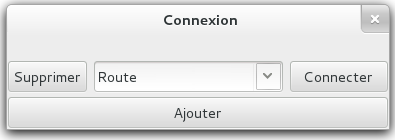
\includegraphics[scale=0.8]{connexion.png}
  \label{connexion}
\end{figure}

\begin{itemize}\setlength{\itemsep}{1mm}
 \item Afin d'accéder à l'écran d'accueil du jeu, il faut sélectionner votre profil dans le menu déroulant puis cliquer sur le bouton "Connecter".
 \item Pour ajouter un nouveau profil, entrez le nom souhaité dans le menu déroulant puis cliquez sur "Ajouter".
 \item Pour supprimer un profil déjà existant, sélectionnez-le dans le menu déroulant puis cliquez sur "Supprimer".
\end{itemize}



\subsection{Accueil}

\begin{figure}[H]
  \center
  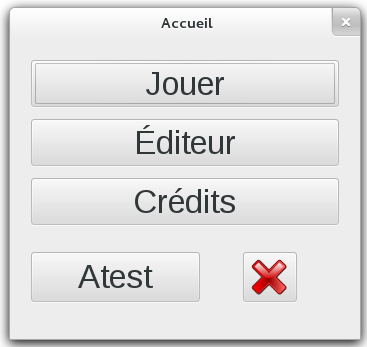
\includegraphics[scale=0.6]{accueil.png}
  \label{accueil}
\end{figure}

\begin{itemize}\setlength{\itemsep}{1mm}
 \item Pour faire une partie de Picross, vous devez cliquer sur "Jouer".
 \item Pour éditer votre propre grille, cliquez sur "Editeur".
 \item Pour consulter les crédits du jeu, cliquez sur "Crédits".
 \item Pour accèdez à vos statistiques ainsi qu'à celles des autres profils, cliquez sur votre pseudo en bas de l'écran.
 \item Pour vous déconnecter et revenir à l'écran de connexion, cliquez sur la croix rouge en bas à droite de l'écran.
\end{itemize}


\subsection{Jeu}
\subsubsection{Choix de la grille}

\begin{figure}[H]
  \center
  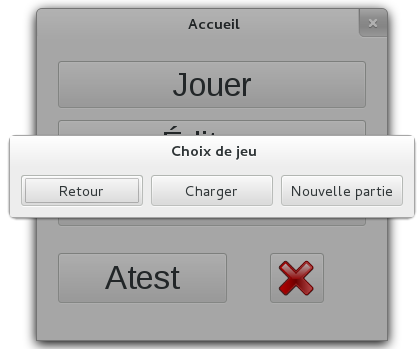
\includegraphics[scale=0.6]{choix_partie1.png}
  \label{accueil}
\end{figure}

\begin{figure}[H]
  \center
  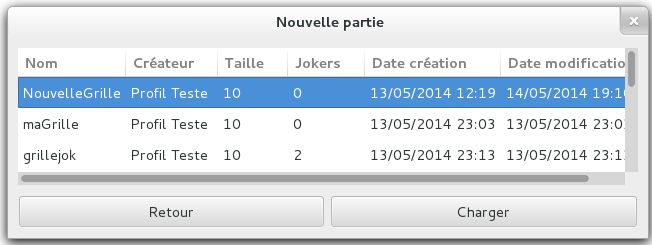
\includegraphics[scale=0.6]{choix_partie2.png}
  \label{accueil}
\end{figure}

\begin{itemize}\setlength{\itemsep}{1mm}
 \item Une fois sur le premier écran, deux options vous sont offertes : reprendre une partie précédemment sauvegardée via "Charger une partie" ou débuter une nouvelle partie via "Nouvelle partie". Vous pouvez également revenir à l'accueil en cliquant sur "Retour à l'accueil".
 \item Quelque soit votre choix lors du premier point, vous arriverez sur le deuxième écran ci-dessus. Dans celui-ci, sélectionnez la sauvegarde ou une des grilles par défaut proposées.
\end{itemize}

\subsubsection{Déroulement de la partie}
\begin{figure}[H]
  \center
  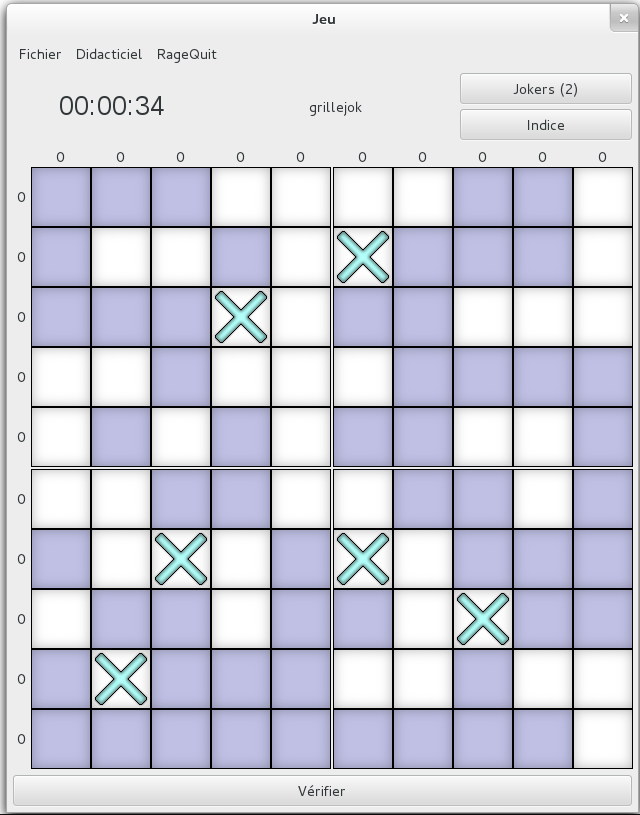
\includegraphics[scale=0.4]{jeu.png}
  \label{jeu}
\end{figure}

\begin{itemize}\setlength{\itemsep}{1mm}
 \item Après avoir choisi votre grille, vous arrivez sur cette interface. Le timer se lance automatiquement. Pour résoudre la grille, la clic gauche noircit les cases et le clic droit sert à barrer une case. Vous disposez également d'indices permettant d'aiguiller votre réflexion et de jokers, dont le nombre est défini par l'éditeur, résolvant une partie de la grille automatiquement mais ajoutant un malus de temps au timer. Lorsque vous pensez avoir résolu la grille, cliquez sur "Vérifier".
 \item Pour sauvegarder une partie en cours, cliquez sur l'option "Sauvegarder" dans "Fichier", rentrez ensuite le nom de sauvegarde de la partie et validez.
\item Pour consulter les règles du jeu et son fonctionnement, cliquez sur "Didacticiel". Tant que la fenêtre du didacticiel est ouverte, le timer est mis en pause.
 \item Pour quitter l'application par accès de fureur, cliquez sur "Ragequit".
 \item Pour revenir à l'écran d'accueil, cliquez sur "Quitter" dans "Fichier". L'application vous demandera avant de quitter si vous souhaitez sauvegarder la partie en cours.
\end{itemize}

\subsubsection{Fin de la partie}

\begin{figure}[H]
  \center
  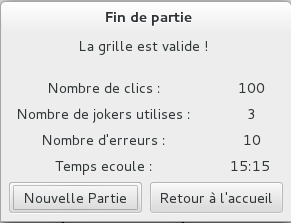
\includegraphics[scale=0.6]{fin_partie.png}
  \label{fin_partie}
\end{figure}

\begin{itemize}\setlength{\itemsep}{1mm}
 \item Une fois la partie terminée et la vérification de la grille validée, vous arrivez sur cet écran. Il affiche vos statistiques concernant cette partie.
 \item Pour lancer une nouvelle partie, cliquez sur "Nouvelle partie".
\item Pour retourner à l'accueil, cliquez sur "Retour à l'accueil".
 \item Pour quitter l'application par accès de fureur, cliquez sur "Ragequit".
\end{itemize}

\subsection{Editeur de grille}

\begin{figure}[H]
  \center
  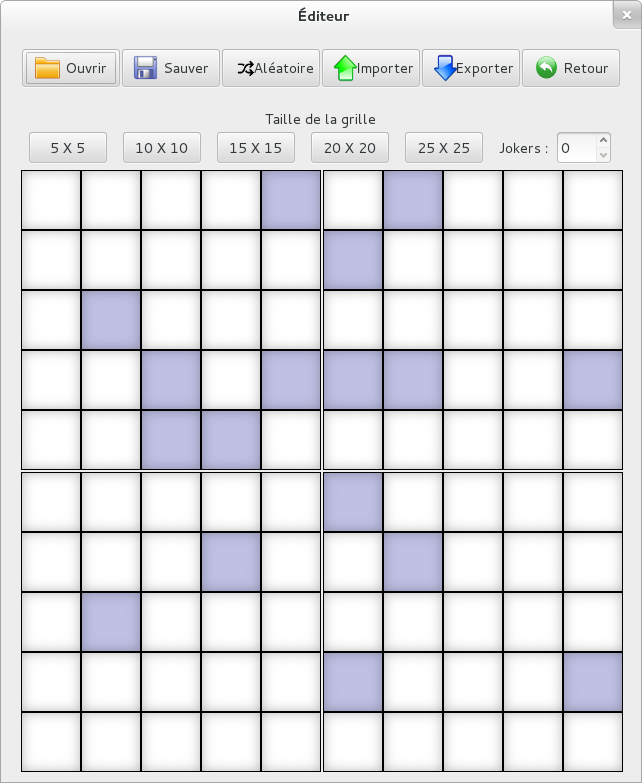
\includegraphics[scale=0.55]{editeur.png}

  \label{editeur}
\end{figure}

\begin{itemize}\setlength{\itemsep}{1mm}
 \item Pour éditer une nouvelle grille, choisissez la taille voulue parmi les 5 choix prédéfinis, saisissez le nombre de jokers utilisables pour la grille et enfin noircissez les cases de la grille à l'aide du clic gauche afin d'obtenir le résultat que vous souhaitez. Une fois cela fait, cliquez sur "Sauver", entrez le nom de la grille et validez.
 \item Pour éditer une grille pré-existante, cliquez sur "Ouvrir", sélectionnez la grille que vous souhaitez modifier et validez. La suite est la même que pour une nouvelle grille.
 \item Pour importer une grille existante d'un autre PC, cliquez sur "Importer" et sélectionner le fichier de sauvegarde correspondant.
  \item Pour créer un fichier exportable d'une grille, cliquez sur "Exporter" , entrez le nom désiré et validez.
 \item Pour noircir une grille de manière aléatoire, cliquez sur "Aléatoire" et un algorithme hautement sophistiqué noircira la grille pour vous.
 \item Pour revenir à l'écran d'accueil, cliquez sur "Retour".
\end{itemize}

\subsection{Statistiques}

\begin{figure}[H]
  \center
  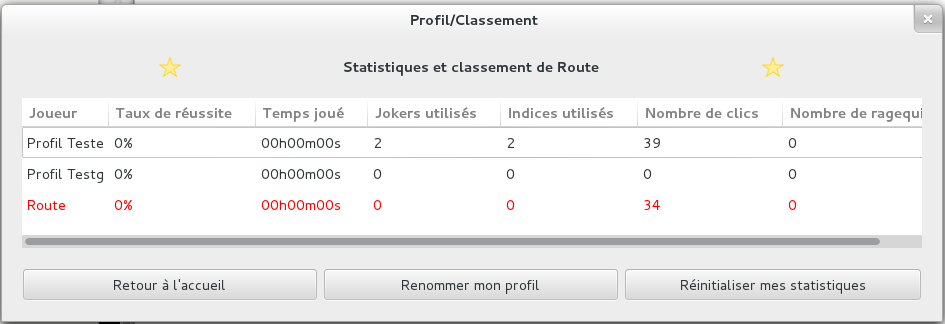
\includegraphics[scale=0.4]{stats.png}
  \label{stats}
\end{figure}

\begin{itemize}\setlength{\itemsep}{1mm}
 \item Sur cet écran vous pouvez consulter les statistiques de chacun des profils existants. Le vôtre est marqué en rouge.
 \item Pour renommer votre profil, cliquez sur "Renommer mon profil", entrez le nouveau nom voulu puis validez.
 \item Pour effectuer une remise à zéro de vos statistiques, cliquez sur "Réinitialiser mes statistiques".
 \item Pour revenir à l'accueil, cliquez sur "Retour à l'accueil".
\end{itemize}

\section{Interactions avec la grille}

\begin{itemize}\setlength{\itemsep}{1mm}
 \item Dans la partie éditeur, le clic gauche sert à noircir les cases. La possibilité de noircir plusieurs cases en cliquant-glissant gauche est également existante. 
 \item Dans la partie jeu, le clic gauche sert à noircir les cases et le clic droit sert à barrer une case. La possibilité de noircir plusieurs cases en cliquant-glissant gauche est également existante. 
 \item Une fois la grille complète, selon vous, cliquez sur "Vérifier".
\end{itemize}

\end{document}
